\documentclass[a4paper,10pt,twocolumn]{jsarticle}
\usepackage{docmute}
\usepackage{myjlababsstyle}
% \usepackage{fancyhdr}
% \usepackage{amsmath,amssymb}
% \usepackage{bm}
% \usepackage[dvipdfmx]{graphicx}
% \usepackage{subfigure}
% \usepackage{url}
% \usepackage{verbatim}
% \usepackage{wrapfig}
% \usepackage{ascmac}
% \usepackage{comment}
% \usepackage{lineno}
% %%%%%%%%%
% \usepackage{myjlababs}


\makeindex
\daigaku{青山学院大学}
\gakubu{社会情報学部}
%\gakka{社会情報学科}
\syubetsu{卒業研究}
%\labname{宮治研究室}
\chiefexaminer{宮治 裕 教授}

%%%%%%%%%%%%%%%%%%%%%%%%%%%%%%%%%%%%%%%
% ここから先「ここまで個人設定」の範囲に
% 各自の固有の情報を記入して下さい
%%%%%%%%%%%%%%%%%%%%%%%%%%%%%%%%%%%%%%%
\nendo{2023年度}
\snum{15387019} %学生番号
\jname{渋谷 太郎} %氏名
\thesistitle{テスト宮治研における論文作成について} %タイトルを記入
\thesissubtitle{\LaTeX の利用} %サブタイトルを記入 ない場合はコメントアウト
\SUBTtrue %サブタイトル有りの場合 ない場合は,コメントアウト
%\SUBTfalse %サブタイトルなしの場合 有りの場合は,コメントアウト
%%%%%%%%ここまで個人設定%%%%%%%%%%%%%%%%%%

\begin{document}
%\linenumbers
\linesparpage{48} %行数指定
%\mojiparline{35} %文字数指定
\maketitle
\thispagestyle{pg}
\pagestyle{pg}

%%%%%%%%%%%%%%%%%%%%%%%%%%%%%%%%%%%%%%%
% ここから先「ここまで本文」の範囲に
% 各自の適切な抄録ファイルを読み込んでください
%%%%%%%%%%%%%%%%%%%%%%%%%%%%%%%%%%%%%%%
\documentclass[a4paper,10pt,twocolumn]{jsarticle}
\usepackage{myjlababsstyle}
\begin{document}
\section{抄録を作成する際の注意事項}
論文抄録とは,簡易なことばで表現すると「論文を要約して書き出したもの」である.
同じように論文を要約した者としては,論文要旨が存在する.
宮治研では節や図表などの論文の体裁に近い形でのものを「抄録」と,節や図表などの情報が記載されていないものを「要旨」とよんで区別している.
社会情報学部では,宮治研でいうところの論文抄録を,論文要旨ということばで指示することがあるため,注意が必要である.

抄録は,論文と同じような見た目ではあるが,その要約の関係から論文の章や節の構成が異なる(ことが多い).
また,論文とは異なる書き方のルールが存在することに注意が必要である.
とくに,抄録内の図表は,そのページの上または下に載せる.
ここで,図表が複数存在する場合には,上下に分散して配置されても良いし,それらが縦方向にまとめて並べられてもよい.

宮治研の卒業研究の抄録(要旨) \LaTeX フォルダには,仕上がりのPDFファイルが配置されている.
そのファイルそのものが,利用方法や利用上の注意を示している.

%
\end{document}
\documentclass[a4paper,10pt,twocolumn]{jsarticle}
\usepackage{myjlababsstyle}
\begin{document}
\section{宮治研~抄録\LaTeX スタイルパッケージの使い方}
基本的に論文のスタイルパッケージと同様に作業をすれば良い.
たとえば,\verb+main.tex+ファイルに必要事項を記載し,適切なファイルを取り込むように指定し,バッチコマンドを利用すれば,PDFファイルができ上がる.

なお,抄録を記述する際注意事項として,スタイルパッケージの利用方法以外については次節にて解説する.

\subsection{サブタイトル有りの場合}
配布したファイルは,サブタイトルがある場合のサンプルになっている.
まず,年度/学籍番号/氏名,タイトル,サブタイトルを所定の命令内に記入する.
\begin{screen}
{\small
%footnotesize
\begin{verbatim}
\nendo{2019年度}
\snum{15387019}
\jname{宮治 裕}
\thesistitle{宮治研における論文作成について}
\thesissubtitle{\LaTeX の利用}
\end{verbatim}
}
\end{screen}
次に \verb+\SUBTtrue+は命令の先頭に\verb+%+がつかない状態に,\verb+\SUBTfalse+は命令の先頭に\verb+%+がつく状態にする.
\verb+%+ が付いているのは,コメントアウト状態であり,コンパイル処理されないことを示す.
\begin{screen}
{\small
%footnotesize
\begin{verbatim}
\SUBTtrue
%\SUBTfalse
\end{verbatim}
}
\end{screen}

\subsection{サブタイトル無しの場合}
サブタイトル有りの場合と比較して3箇所の変更が必要である.
\begin{enumerate}
\item サブタイトルを記入する命令の先頭部分に \verb+%+ 記号を入れ,コメントアウト状態にする
\item \verb+\SUBTtrue+の前に\verb+%+ 記号を入れ,コメントアウト状態にする
\item コメントアウト状態の \verb+\SUBTfalse+の直前の \verb+%+ 記号を削除する
\end{enumerate}
以上の変更を行った設定を示す.
\begin{screen}
{\small
%footnotesize
\begin{verbatim}
%\thesissubtitle{}
%\SUBTtrue
\SUBTfalse
\end{verbatim}
}
\end{screen}

%
\end{document}
\documentclass[a4paper,10pt,twocolumn]{jsarticle}
\usepackage{myjlababsstyle}
\begin{document}
\section{基本的な入力方法}
\LaTeX を利用する際に,最初に知っておくべきことは「スペース」や「改行」などが,エディタで入力したとおりにならないことと,キーボード上の記号の中には 「\%」 など,そのまま入力しただけでは出力できない文字が有るということである\footnote{ちなみに\%記号を表示したい場合は,「\verb+\%+」と入力する}.
これらのポイントは,電気通信大学 佐藤研究室による「TeXマニュアル」\cite{HTUlatex}にまとめられている.

以降,特に注意するポイントについてのみ記載する.
\subsection{章と節,節々}
章のタイトルには \verb+\chapter{}+,節のタイトルには \verb+\section{}+を利用する.
また,節の下のレベル(ここでは節々) のタイトルを記載するには \verb+\subsection{}+を利用する.
それぞれ,適切なフォーマットにて番号が付与されて,表示がなされる.

更に下のレベルは,\verb+subsubsection{}+を用いることができる.本スタイルパッケージでは,
このレベルにおいて番号を記載しないようにした.
したがって,このレベルを最小として論文を構成するようにして欲しい.

なお後述の理由から,抄録では \verb+\chapter{}+は利用しない.
.

\subsection{改行と改段落}
\LaTeX では,HTMLを書くときと同様に,エディタ上で「半角空白をいくついれたか」「改行したか」といった情報は,無視される.

改行には 「\verb+\\+」を,改段落には 「\verb+\par+」を利用する\footnote{改段落の場合には「\verb+\par+」を入れるのではなく,空白行を入れる方法を推奨するが,説明として記載している}\footnote{改段落された後の段落は,自動的に一字下げされる.一方で改行の場合には,字下げはなされない.}\footnote{どうしてもスペースを空けたい場合には,「\verb+~+」を利用する.}.

一見不自由に見えるかもしれないが,この特性は論文を書く際に便利な機能である.
まず,論文を書く際に,意図的な改行を入れることはあまりない.
つまり改行の 「\verb+\\+」を使うことは,ほとんど無い.

逆に改段落は,論文を書く際には意識して頻繁に利用する.
ここで,段落が変わる位置に空白行を挿入すると,「\verb+\par+」と入力したことと同じ意味となる.
%したがって,改段落には \verb+\par+を入れるのではなく,空白行を入れる方法を推奨する.

テキストエディタなどで文章を書く際のポイントと効果を以下にまとめる.
\begin{itemize}
\item 一文ずつ改行しながら文章を記述する
\begin{itemize}
\item[・] 行がつながっていない方が,エディタ上の編集では効率的である
\item[・] 改行は,文章の仕上がりの見た目の改行ではない
\end{itemize}
\item 段落が変わる毎に空白行を挿入する
\begin{itemize}
\item[・] エディタ画面では,段落のまとまりがわかりやすい
\item[・] 文章のバランスや量などに気を配ることができる
\end{itemize}
\end{itemize}

\begin{comment}
上記ポイントを実践して記述した本書類の第1章の中身を以下に示す.
\begin{screen}
{\footnotesize
\begin{verbatim}
\section{はじめに}
本論文では,○○○を△△△することにより,□□を明らかとする研究について記述する.

まず,本研究をおこなう背景となった事柄について述べる.
次に,研究目的の詳細を記述した後,類似研究との相違や関連研究とのつながりについて解説する.
また,次章以降の本論文の構成についてその概略を述べる.

\subsection{背景}
研究の目的につながる背景事項を説明する.
その説明には,参考文献やデータを参照するように.

あまり詳しく書きすぎると,2章や3章などで書く内容が無くなったり重複したりしてしまうので,研究の目的の妥当性につながる程度の内容(詳細さ)でかまわない.

\subsection{研究目的}
背景によって,研究の大きな目的が導かれる.
その大きな目的を正確に定義した後,本研究にて実際にターゲットとする目的を詳細に記述する\footnote{大きな目的は1年間の研究ではカバーしきれない為}.

また,背景にて実際の詳細なターゲットの必要性を示した場合には,それの詳細な条件を記載する.
…
\end{verbatim}
}
\end{screen}
\end{comment}
%
\end{document}
\documentclass[a4paper,10pt,twocolumn]{jsarticle}
\usepackage{myjlababsstyle}
\begin{document}
\section{\LaTeX で抄録を作成する上での注意事項}
\LaTeX ので抄録を作成するうえでの注意事項について,主要なポイントについて記す.

\subsection{一番大きな文章単位: 節}
論文と抄録では,文章を作成する際のスタイルファイルが異なる.
宮治研の\LaTeX スタイルパッケージにおいて,論文では\verb+jsbook.cls+を,抄録においては\verb+jsarticle.cls+を用いている.

ここで,\verb+jsarticle.cls+を利用する際には,「章(\verb+\chapter{}+)」を利用することができない.
したがって,一番大きな枠組みとして「節(\verb+\section{}+)」を利用することになる.

\subsection{図表の位置の指定}
論文を書く際には,図や表の位置は本文中の記載よりも後であれば,とくに気にする必要はなかった.
そのため,\verb+\begin{figure}[htbp]+の様に記述し,h(この場所)t(ページ上部)b(ページ下部)p(1ページ)の順の優先順位で図の位置を指定していた.

しかし,抄録の場合,図や表の位置は論文の上部や下部にまとめる.
その為,\verb+\begin{figure}[b]+もしくは\verb+\begin{figure}[t]+のように指示をする必要がある.

なお,図の文字サイズは,本サンプルファイル程度の小ささが限界と考えること.

\begin{screen}
{\small
\begin{verbatim}
\begin{figure}[b]
\centering
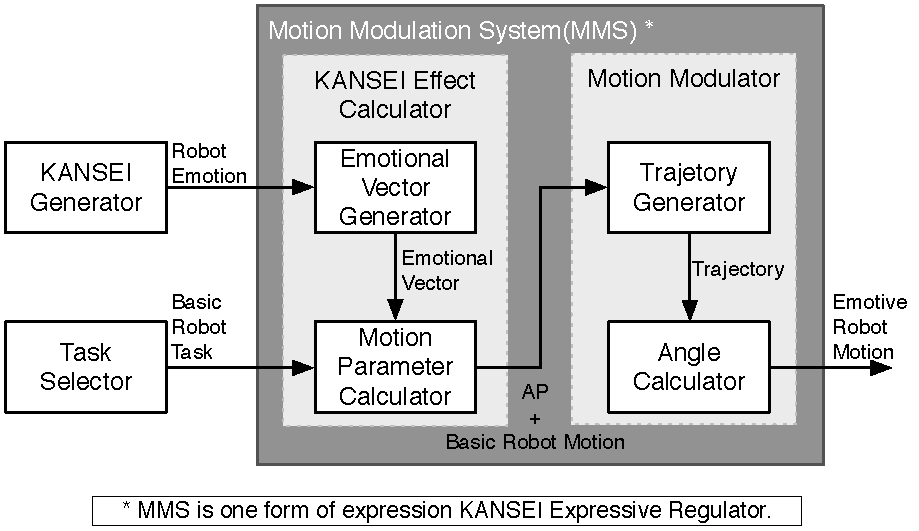
\includegraphics[width=8cm]{MMS.pdf}
\vspace{-7mm}
\caption{MMSの内部構成}
\label{fig:mms}
\vspace{2mm}
\end{figure}
\end{verbatim}
}
\end{screen}

\begin{figure}[b]
    \centering
    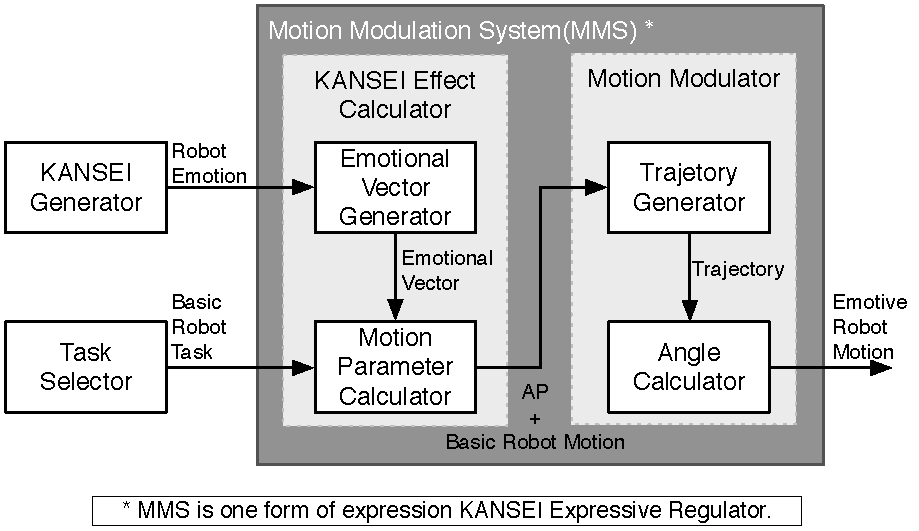
\includegraphics[width=8cm]{MMS.pdf}
    \vspace{-7mm}
    \caption{MMSの内部構成}
    \label{fig:mms}
    \vspace{5mm}
\end{figure}

\subsection{参考文献について}
抄録においては,参考文献のフォーマットも省略することが多いのだが,今回は論文時と同様の表記にて提出することとした.

参考文献を記載するファイルは新たに作成せず,論文と同じ \verb+myrefs.bib+ファイルをスタイルパッケージのフォルダにコピーし,しかるべき引用命令を入れれば良い.
サンプルとして,論文\cite{Kogami2009},書籍(の一部)\cite{WelfareJapan},書籍\cite{Nakata2010},予稿集\cite{Miyaji2003ROMAN},その他(Webサイトなど)\cite{HTUlatex}を組み込んだ.

%
\end{document}

\documentclass[a4paper,10pt,twocolumn]{jsarticle}
\usepackage{myjlababsstyle}
\begin{document}
\section{その他}
その他の事項として、本節では表の記述方法とぶち抜きの図について記載する。

\subsection{表の記述}
論文を記述する際にも指摘したが、表においては数値は右詰にしなければならない。
また、ラベル部は中央揃えとすることが多い。

そのような設定をしたものを、表~\ref{table:face_rec}に示す。

\begin{table}[b]
\centering
\vspace{2mm}
\caption{WHLACによる顔表情認識率}
\label{table:face_rec}
\vspace{3mm}
\small
\begin{tabular}{r|r|r|r} \hline
\multicolumn{1}{c|}{Data \#} & \multicolumn{1}{c|}{Ave.} & \multicolumn{1}{c|}{Max.} & \multicolumn{1}{c}{Min.} \\ \hline\hline
1 &  0.67 (N/A) & 0.91 (39) & 0.46(21) \\ \hline
2 & 0.37 (N/A) & 0.50 (38) & 0.09(10) \\ \hline
3 & 0.65 (N/A) & 0.87 (45) & 0.28(10) \\ \hline\hline
\multicolumn{1}{c|}{Total Ave.} & 0.56 & 0.76 & 0.27 \\ \hline
\end{tabular}
\end{table} %

\subsection{二段ぶち抜きの図}
二段組の省略ではあるが、図表の設定(開始タグと終了タグを共に)を~\verb+figure*+ とすることで、左右の段をぶち抜いて図表を入れることができる。
例を図\ref{fig:mp2}に示す。

\begin{screen}
{\small
\begin{verbatim}
\begin{figure*}[bt]
\centering
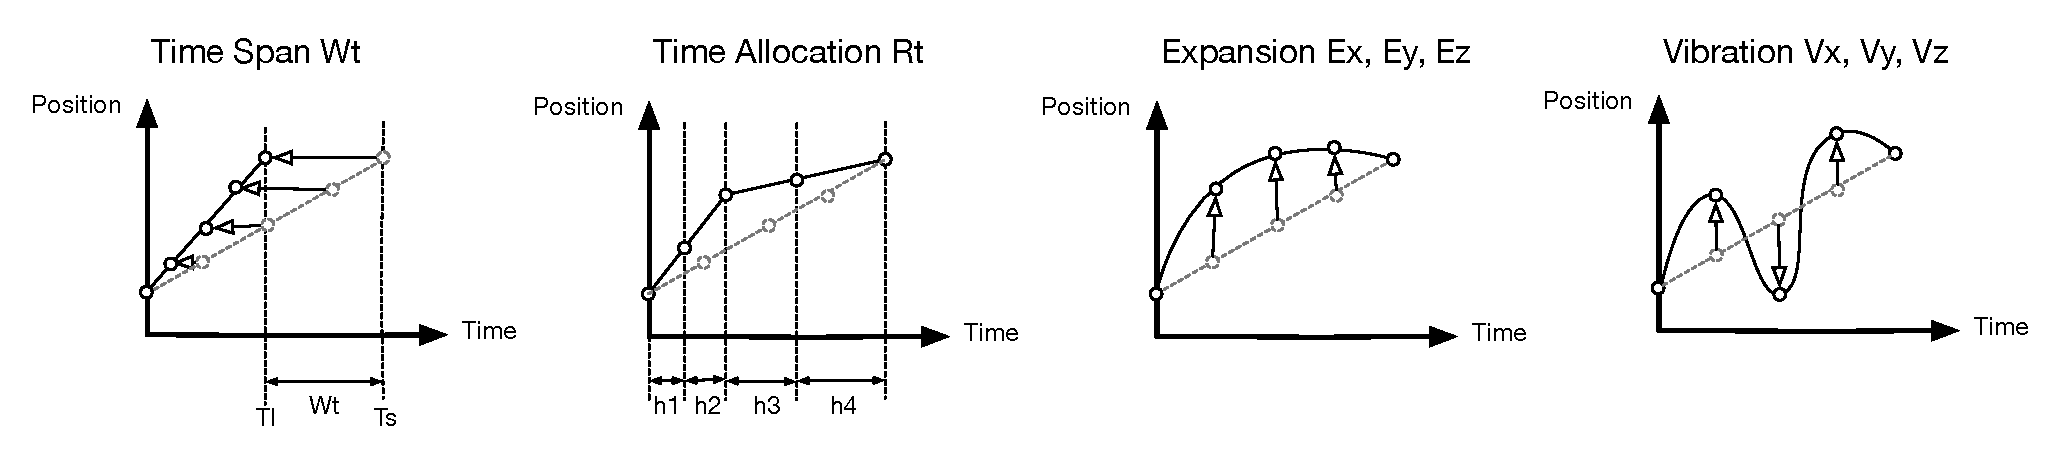
\includegraphics[width=14cm]{mp2.pdf}
\vspace{-7mm}
\caption{MMSの内部構成}
\label{fig:mp2}
\vspace{5mm}
\end{figure*}
\end{verbatim}
}
\end{screen}

\begin{figure*}[bt]
    \centering
    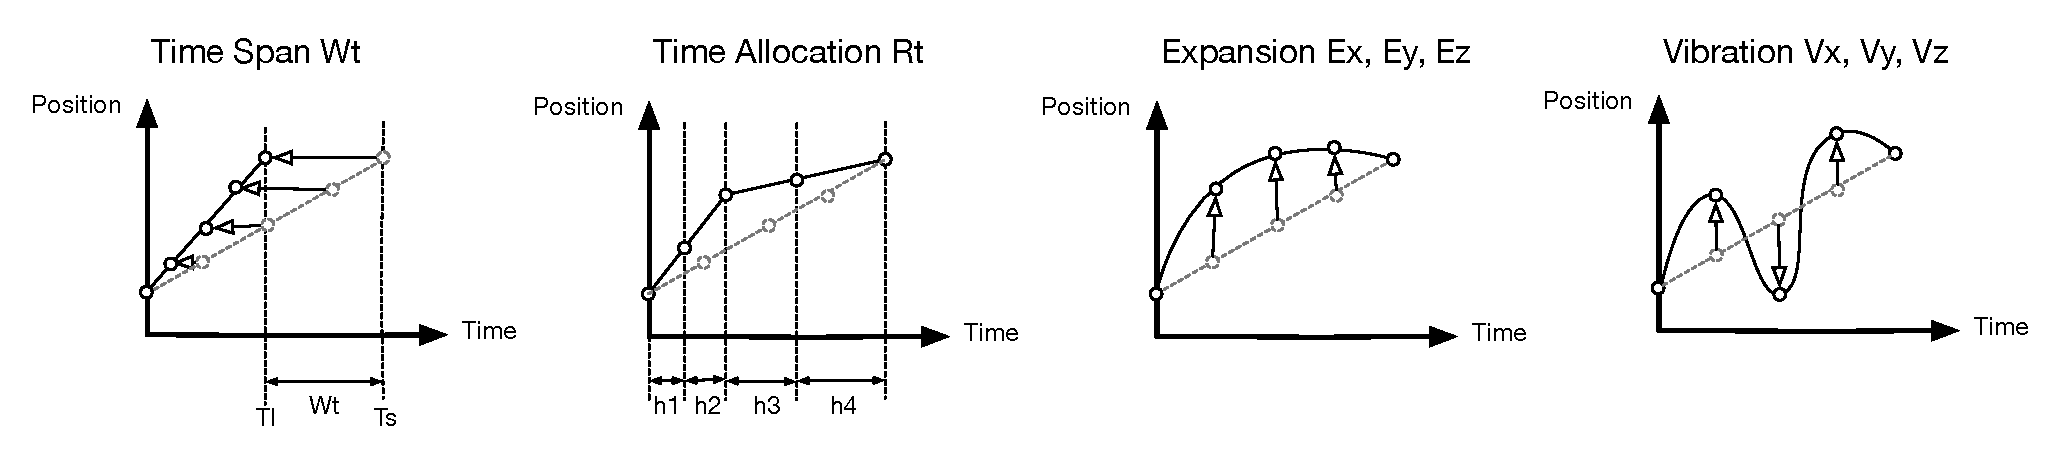
\includegraphics[width=18cm]{mp2.pdf}
    \vspace{-7mm}
    \caption{MMSの内部構成}
    \label{fig:mp2}
    \vspace{5mm}
\end{figure*}



%
\end{document}
\documentclass[a4paper,10pt,twocolumn]{jsarticle}
\usepackage{myjlababsstyle}
\begin{document}
\section{Visual Studio Codeで編集する人へ}
Visual Studio Codeを使って \LaTeX 論文を作成する人が増えているため,それに合わせた修正を各所でおこなっている.
以下の設定や,注意事項を参照してほしい.

\subsection{コンパイルのための設定}
\LaTeX をコンパイルする際には,目次や参照,参考文献などを組み込むための処理などを複数回実行する必要がある.
これを自動で判断して実行するための設定ファイルが \verb+.latexmkrc+である.
本スタイルファイルパッケージでは,以下の設定をしている.
\begin{screen}
{\small
\begin{verbatim}
#!/usr/bin/env perl
$pdf_mode = 3;
$latex = 'platex -halt-on-error';
$bibtex = 'pbibtex';
$dvipdf = 'dvipdfmx %O -o %D %S';
\end{verbatim}
}
\end{screen}

なお,一部の行を割愛して表示している.
詳細は,直接ファイルを確認してほしい.

\subsection{LaTeX Workshop の設定}
VSCodeプラグインであるLaTeX Workshopの設定は,以下の様にしている.
なお,必ずしも同じ設定にする必要はない.
\begin{screen}
{\footnotesize
\begin{verbatim}
"latex-workshop.latex.tools": [
  {
    "name": "Latexmk (pLaTeX)",
    "command": "latexmk",
    "args": [
      "-f",
      "-gg",
      "-pv",
      "-latex='platex'",
      "-synctex=1",
      "-interaction=nonstopmode",
      "-file-line-error",
      "%DOC%"
    ]
  },
],
\end{verbatim}
}
\end{screen}
\begin{screen}
    {\footnotesize
    \begin{verbatim}
"latex-workshop.latex.recipes": [
  {
    "name": "pLaTeX",
    "tools": [
      "Latexmk (pLaTeX)"
    ]
  },
],
\end{verbatim}
}
\end{screen}
\begin{screen}
{\footnotesize
\begin{verbatim}
"latex-workshop.latex.magic.args": [
  "-f",
  "-gg",
  "-pv",
  "-synctex=1",
  "-interaction=nonstopmode",
  "-file-line-error",
  "%DOC%"
],
\end{verbatim}
}
\end{screen}
\begin{screen}
{\footnotesize
\begin{verbatim}
"latex-workshop.view.pdf.viewer":"tab",
"latex-workshop.latex.autoBuild.run": "never",
"latex-workshop.view.pdf.refviewer":"tabOrBrowser",
"latex-workshop.latex.autoClean.run":"onBuilt",
\end{verbatim}
}
\end{screen}

\subsection{分割(子ファイル)コンパイル}
通常の \LaTeX のファイルの場合に親ファイルに記述する文書開始や終了/スタイルファイルの読み込みを子ファイル側に書き込むことによって,それぞれのファイルごとにコンパイルができる.

\begin{screen}
{\footnotesize
\begin{verbatim}
\documentclass[a4paper,10pt,twocolumn]{jsarticle}
\usepackage{myjlababsstyle}
\begin{document}
\section{これは読み込まれる子ファイルの例}
ファイル名は sub.tex とします.
\end{document}
\end{verbatim}
}
\end{screen}

これを読み込む親ファイル側では,これらの設定を無視するようにしなければならない.
そのために,\verb+docmute+パッケージを用いている.
親ファイルの例を以下に示す.
\begin{screen}
{\footnotesize
\begin{verbatim}
\documentclass[a4paper,10pt,twocolumn]{jsarticle}
\usepackage{docmute}
\usepackage{myjlababsstyle}
\begin{document}
これは親ファイルの例です.
\input{sub}
\end{document}
\end{verbatim}
}
\end{screen}

また,多くのスタイルファイルを親ファイルと子ファイルで共通して読み込むために,スタイルファイルを \verb+myjlababsstyle.sty+ ファイル内に列挙している.
各自でスタイルファイルを追加する場合には,このファイルに記載すること.

\subsection{テキスト校正くん}
「テキスト校正くん」パッケージは追加すべきである.
ただし,\LaTeX のファイルは校正してくれないため,\verb+txt+か\verb+md+のファイルを作成し,そこに文章を貼り付けて校正するのが良い.
インストールや設定などが必要ない「テキスト校正くん」を利用することにしたが,昨年まではRedpenと比較して細かい部分の校正は不十分である.
最低限の校正として必ず利用してほしい.
%
\end{document}
\documentclass[a4paper,10pt,twocolumn]{jsarticle}
\usepackage{myjlababsstyle}
\begin{document}
\section{システム構成図の例}
システム構成図が論理的に描けると,論文そのものの説明もしやすくなる.
ここでは,シスム構成図の例をいくつか記載する.
\begin{figure}[t]
  \centering
  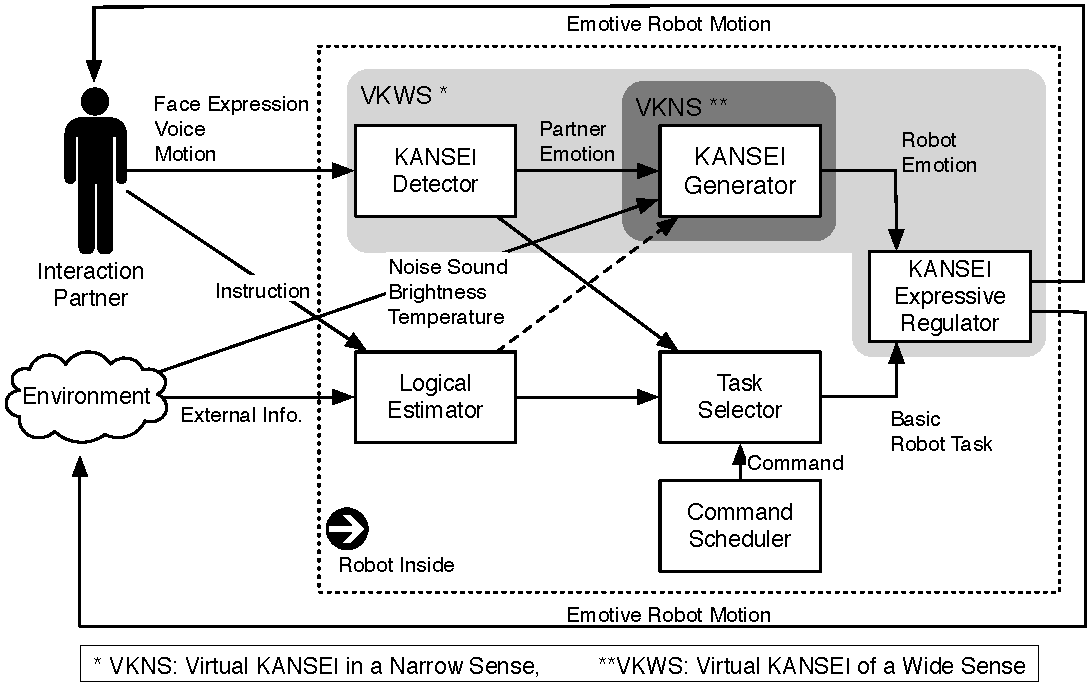
\includegraphics[width=9cm]{VKall.pdf}
  \vspace{-7mm}
  \caption{擬似感性の構成}
  \label{fig:vkall}
  \vspace{5mm}
\end{figure}

\begin{figure}[t]
  \centering
  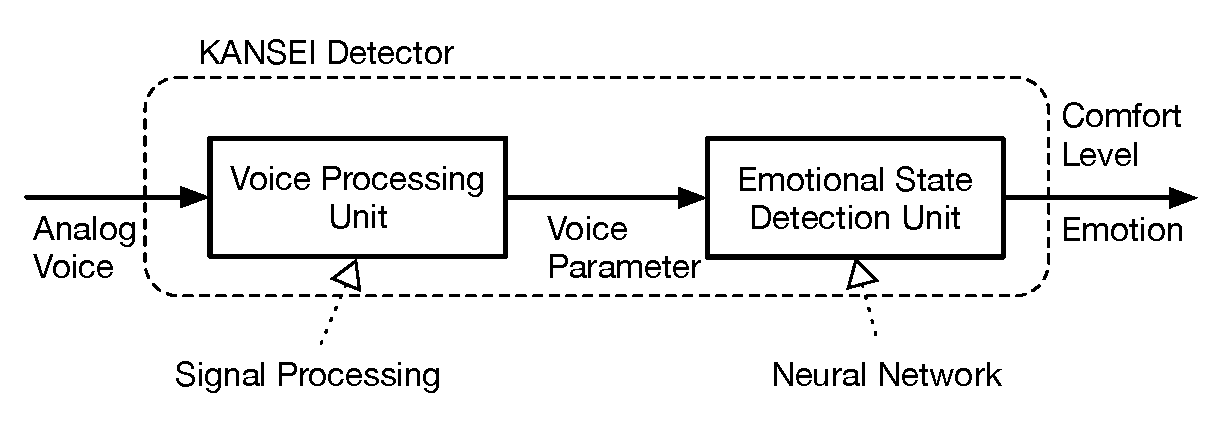
\includegraphics[width=8cm]{VoiceKANSEIDetector.pdf}
  \vspace{-7mm}
  \caption{音声からの感性同定部}
  \label{fig:VoiceKANSEIDetector}
  \vspace{5mm}
\end{figure}

%
\end{document}

%%%%%%%%ここまで本文%%%%%%%%%%%%%%%%%%%%%%

\bibliographystyle{junsrt}
\bibliography{myrefs}
% myrefs.bib の中はサンプルファイルを参考に記述
%
\end{document}
